The main challenge is that there is currently no way to express an optimality of an edge flow by one number, which is critical for learning methods when we want to compute a loss function. We previously mentioned that an optimal flow has uniformly distributed points, edge lenghts and overall area of a primitive. One way to possibly achieve that is to look at the task at hand from different perspective. Instead of doing a correction of the given 3D mesh, we will try to reconstruct the shape of a given 3D mesh with better topology.

In this chapter we will explore researches using neural networks for 3D mesh reconstruction. 

\section{Retrieve and deform a template}

Retrieve and deform a template is a two step solution. First a most suitable template is picked and then it is deformed to the target object. The input is processed with neural network which classifies which template is best suited, such as BCNet \cite{bcnet}, MultiGarment Net\cite{mgn} or ShapeFlow \cite{shapeflow}. As seen in Figure \ref{fig:bcnet} and \ref{fig:shapeflow}, a nearest-neighbor template is retrieved from the embedded space and then a deformation network is applied.

\begin{figure}[h]
    \centering
    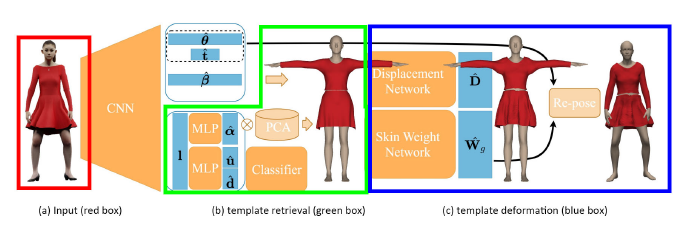
\includegraphics[width=12cm]{bcnet.png}
    \caption{Overview of retrieve and deform shape reconstruction using BCNet \cite{bcnet}}
    \label{fig:bcnet}
\end{figure}

\begin{figure}[h]
    \centering
    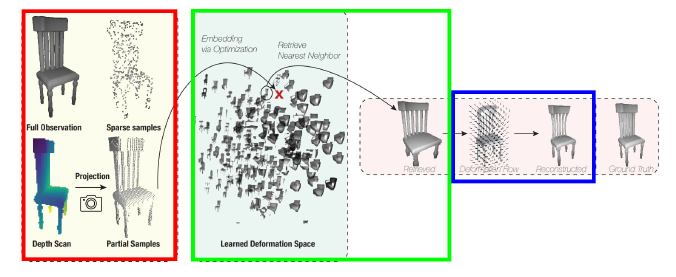
\includegraphics[width=12cm]{shapeflow.png}
    \caption{Overview of retrieve and deform shape reconstruction using ShapeFlow \cite{shapeflow}}
    \label{fig:shapeflow}
\end{figure}

\section{Deform a primitive}

Retrieve and deform solution expects a high quality templates and they were also highly specialized in certain category type, which makes the overall input and output then highly specialized. Other method often used for aproximating to target object from a single image would be deforming a primitive. Popular representation in Pixel2Mesh \cite{p2m}, Pixel2Mesh++ \cite{p2mpp}, Neural mesh flow \cite{neuralFlow} was a simple sphere. 

Pixel2Mesh had a 2D CNN extracting features from a single image which is then leveraged by a deformation block, progressively deforming a sphere into the desired 3D model. The cascaded mesh deformation network is a graph-based convolution network, containing three deformation blocks intersected by two graph unpooling layers, which increases the number of vertices. With given face the points were added to the middle of each connecting edges. Connecting these newly added points then forms a new set of primitive faces, while also ensuring even distribution of vertices and their degrees. The improved Pixel2Mesh is extracts features from multiple view images, increasing the reconstruction accurancy. 

\begin{figure}[h]
    \centering
    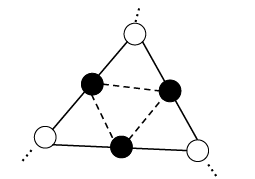
\includegraphics[width=6cm]{p2m_unpooling.png}
    \caption{Graph unpooling\cite{p2m}}
    \label{fig:p2munpooling}
\end{figure}

\begin{figure}[h]
    \centering
    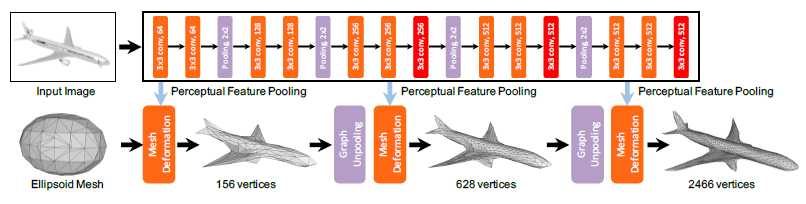
\includegraphics[width=12cm]{p2m.png}
    \caption{Pixel2Mesh architecture overview \cite{p2m}}
    \label{fig:p2m}
\end{figure}

The Neural mesh flow shares very similar architecture as Pixel2Mesh in using three deform blocks.

Neural Mesh Flow (NFM) as seen in Figure \ref{fig:netflow}, learns to auto-encode 3D shapes. NMF broadly consists of four components. First, the target shape is encoded by uniformly sampling N points from its surface and feeding them to a PointNet \cite{pointnet} encoder to get the global shape embedding. Second, NODE blocks diffeomorphically flow the vertices of template sphere towards target shape conditioned on shape embedding. Third, the instance normalization layer performs non-uniform scaling of NODE output to ease cross-category training. Finally, refinement flows provide gradual improvement in quality.

\begin{figure}[h]
    \centering
    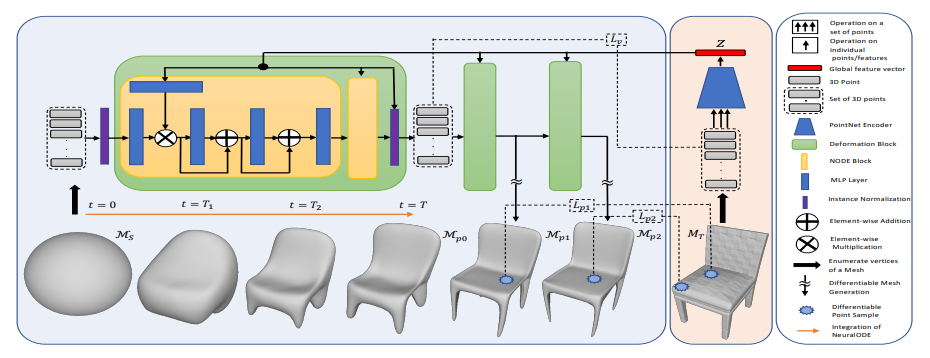
\includegraphics[width=12cm]{netflow.png}
    \caption{Neural Mesh flow architecture overview \cite{neuralFlow}}
    \label{fig:netflow}
\end{figure}




The mesh reconstruction is often done from voxels, point clouds, single images, and multi-view images, respectively. There was previously no real purpose of doing a reconstruction from a mesh as in our case.

universal solution, depends on previous topology quality